\chapter{\uppercase{$^{227}$Ac as a Calibration Source}} \label{ch:Ac}

\section{Motivation}

In the absence of an eV-scale sterile neutrino PROSPECT should measure IBD rates that fall like one over distance from the reactor squared. 
If sterile neutrino oscillation was detected, after one year PROSPECT would measure the spectrum seen in Figure~\ref{fig:lovere1yr}, given a mass splitting of 1.78 eV$^2$, .
However, a situation could occur in which a sterile neutrino did not exist, or could not be measured with PROSPECT, and an oscillation is still measured.
This could happen if there are segment to segment volume variations throughout the detector, mimicking an oscillation signal.
Therefore, it becomes important that the product of efficiency$\times$volume for all segments is well known. 

\begin{figure}[h]
	\centering
	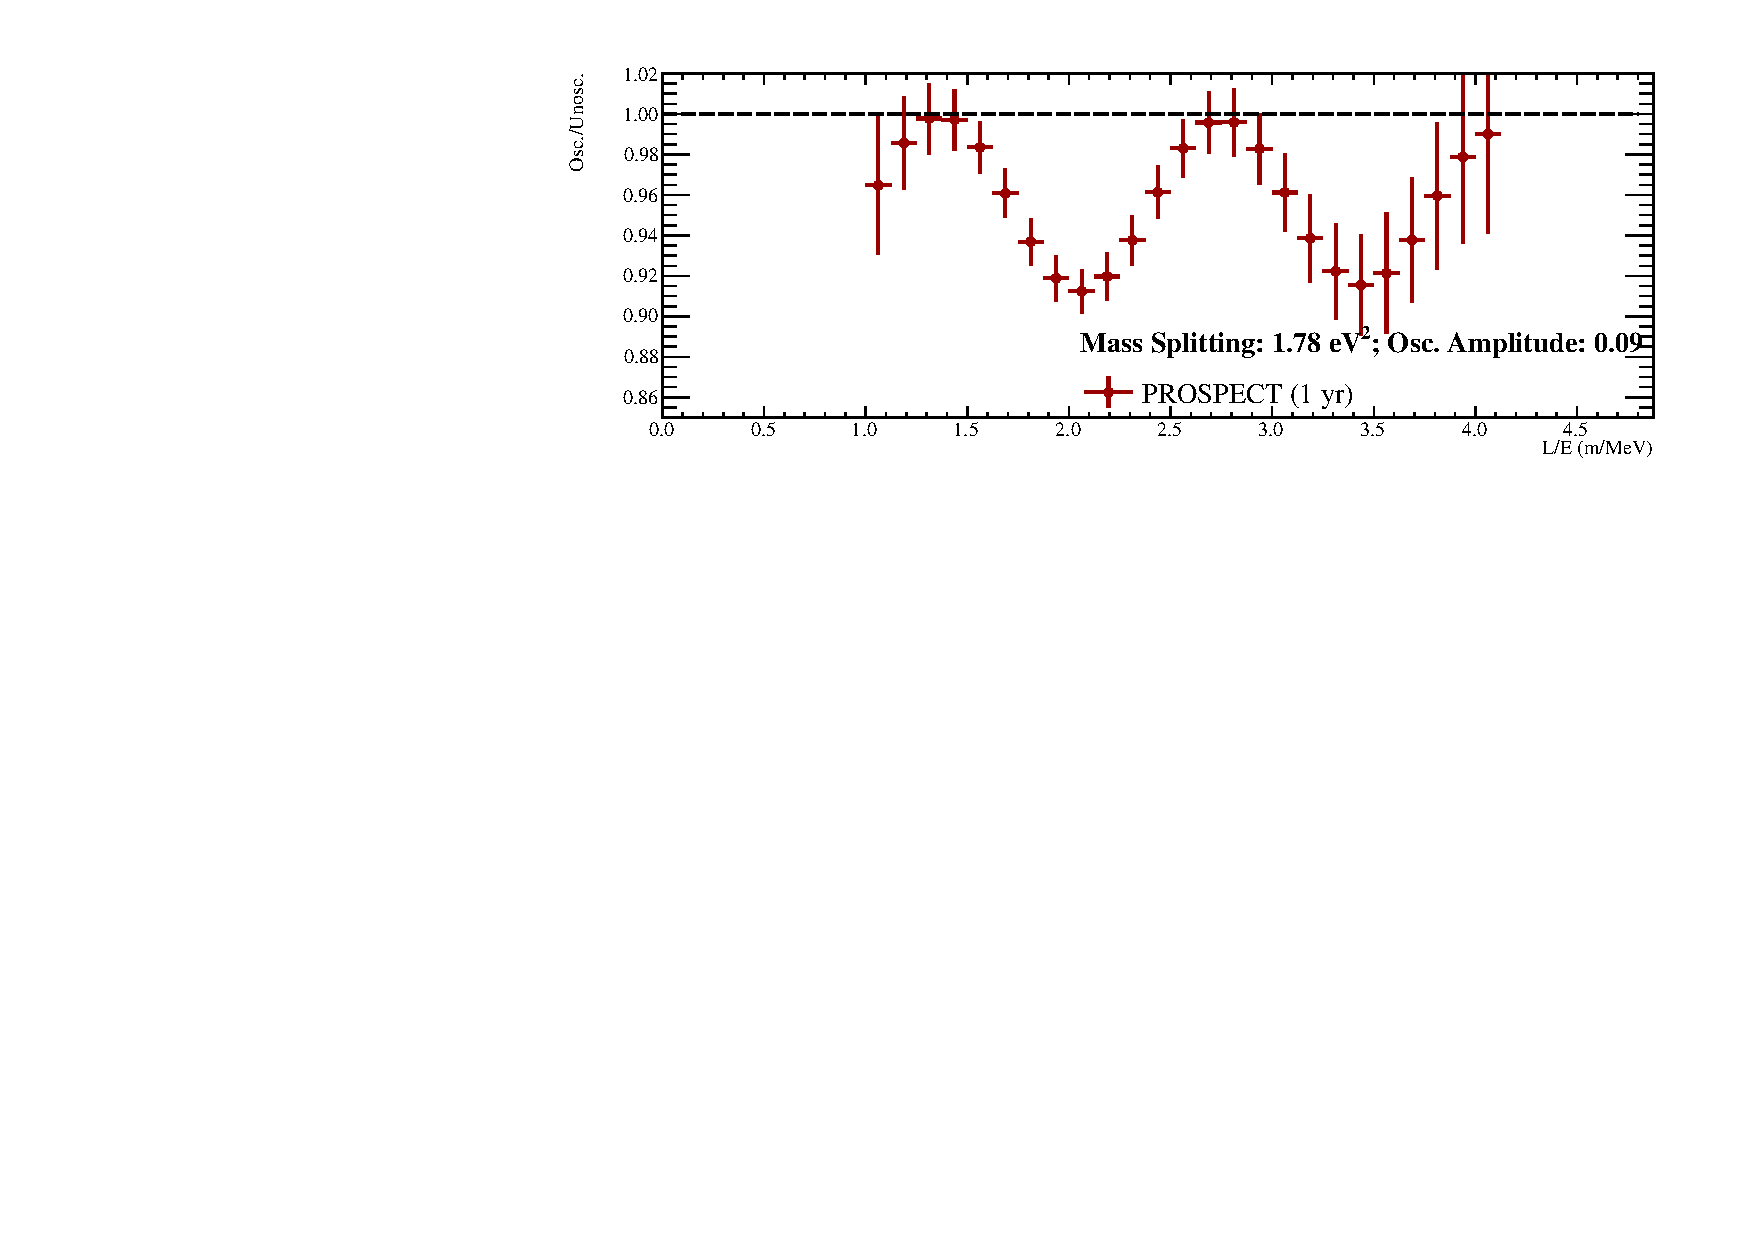
\includegraphics[width=0.7\linewidth]{tex/6-ac227-images/LoverE_1yr}
	\caption[Monte Carlo neutrino spectrum as a function of L/E]{The ratio of the oscillated to un-oscillated neutrino spectrum as a function of L/E that would be observed by PROSPECT after 1 year if a sterile neutrino signal was detected \cite{PSurukuchi:1534}.}
	\label{fig:lovere1yr}
\end{figure}


This measurement can be accomplished if an event source is uniformly distributed throughout the active volume of the detector. 
By measuring the rate of this source in each segment the relative volumes can be compared and tracked through time.
\Ac was chosen as the source and a chloride solution was prepared and dissolved in the liquid scintillator to ensure uniform distribution.

\Ac was chosen for several reasons. First, because an \AaAa coincidence occurs in its decay chain, specifically $^{219}$Rn $\rightarrow ^{215}$Po + $\alpha \rightarrow ^{211}$Pb + \Aa, as highlighted in Figure~\ref{fig:ac227chain}.
\Rn has a half-life of 3.96 $\pm$ 0.01 s and $\alpha$-decays 100\% of the time, while \Po has a half-life of 1.781 $\pm$ 0.005 ms and $\alpha$-decays  99.99977(2)\% of the time \cite{ENSDF}, so the \AaAa coincidences happen frequently.
The \Aa decay of \Po is mono-energetic at 7.39 MeV which results in a $\sim$0.78 MeVee signal after quenching, well removed from nLi captures that occur around 0.5 MeVee. 
In addition, there are no corresponding gammas with the \Po decay, making this a very clean and well defined signal.
The \Rn \Aa decays are not so nice, as there are four dominant alpha energies and three dominant gamma energies for these decays, as listed in Table~\ref{tab:RnPoE}, but the use of time, energy, and PSD cuts make them easy to pair with corresponding \Po decays.

\begin{figure}[hb]
	\centering
	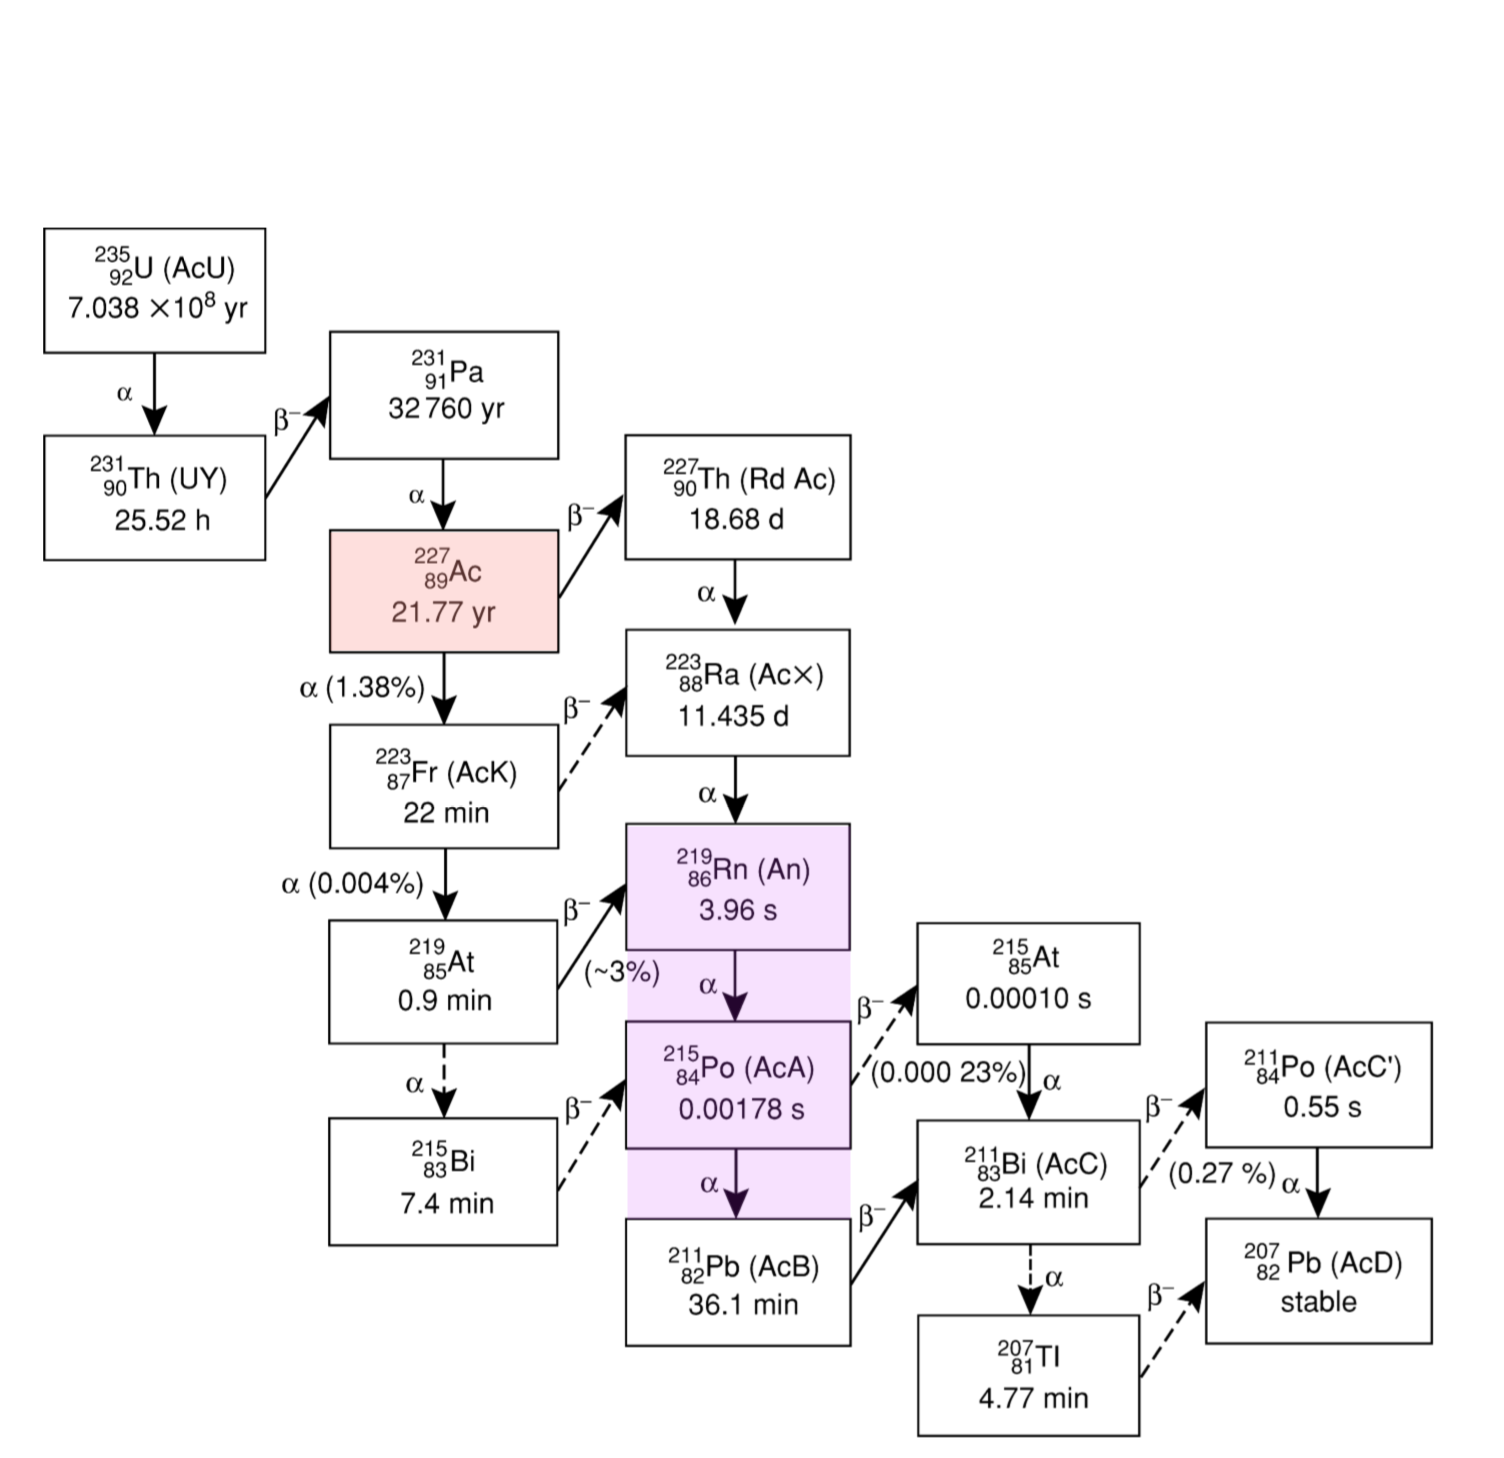
\includegraphics[width=0.6\linewidth]{tex/6-ac227-images/Ac227Chain}
	\caption[\Ac decay chain]{The full decay chain of \Ac (a daughter of $^{235}$U), in which the \AaAa coincidence of interest is highlighted \cite{Kirby2011}.}
	\label{fig:ac227chain}
\end{figure}

\begin{table}[h]
	\centering
\begin{tabular}{|c|c|c|c|c|c|}
	\hline 
	& E$_\alpha$ [keV] & I$_\alpha$ \% &  & E$_\gamma$ [keV] & I$_\gamma$ \% \\ 
	\hline 
	\Rn & 6425.0(10) & 7.5(6) &  & 271.23(1) & 10.8(6) \\ 
	%\hline 
	& 6530(2) & 0.110(10) &  & 401.81(1) & 6.6(4) \\ 
	%\hline 
	& 6552.6(10) & 12.9(6) &  & 130.60(3) & 0.13(9) \\ 
	%\hline 
	& 6819.1(3) & 79.4(10) &  &  &  \\ 
	\hline 
	\Po & 7386.1(8) & 99.999770(20) &  &  &  \\ 
	\hline 
\end{tabular} 
\caption[$\alpha$ and $\gamma$ energies of \Rn and \Po decays]{Energy and absolute intensity of dominant $\alpha$ and $\gamma$ decay radiation for \Rn and \Po. Decay energies not listed here have an intensity of $< $0.05\%.}
\label{tab:RnPoE}
\end{table}

%\begin{figure}[h]
%	\centering
%	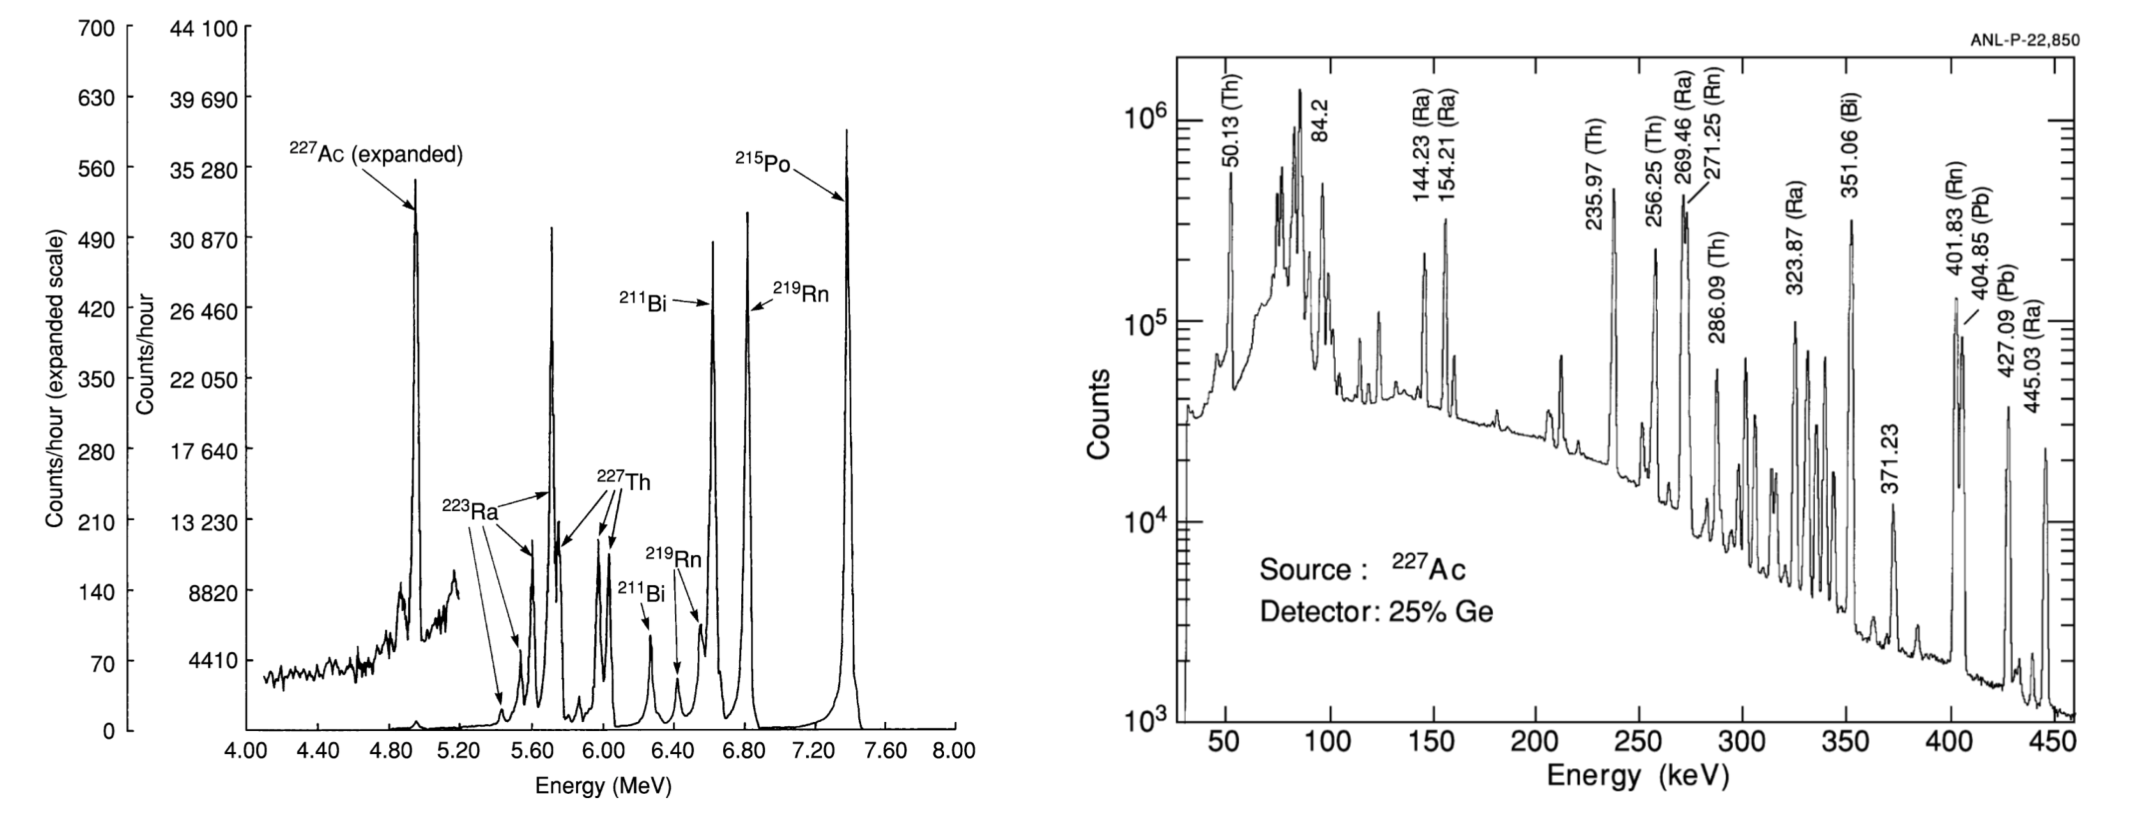
\includegraphics[width=0.95\linewidth]{tex/6-ac227-images/Actinium_agSpectrum}
%	\caption[]{\cite{Kirby2011}}
%	\label{fig:actiniumagspectrum}
%\end{figure}


\section{Material Compatibility}

Before \Ac could be added to the PROSPECT detector, it had to be determined that \Ac and its daughters would not adsorb onto detector materials.
If it was adsorbed then it would not be a uniform source in the detector, nullifying its use as a method to track relative efficiency$\times$volume throughout the detector.
To test this six material samples were placed in vials of $^6$Li-LS spiked with \Ac. The rate of \Ac in each sample vial and one reference vial with no material was measured and tracked over a period of 6 months. 
An observation of a significant decrease in rate, relative to the half-life of \Ac, would indicate that \Ac was adsorbing onto the material.

\subsection{Material and Scintillator Preparation}
The materials tested were: ultraviolet transmitting (UVT) acrylic, flourinated ethylene propylene (FEP), polylactide (PLA), polyether ether ketone (PEEK), a RG 188 cable, and viton o-rings. See Table~\ref{tab:materials} for a list of their uses in the detector and sample sizes.
To prepare the materials they were all placed in a single beaker with ultra-pure water and cleaned ultrasonically for 30 minutes.
They were then transferred to a watch glass and placed in a 50 C over for two hours.
After drying they were placed in empty 12 mL vials.

The \Ac used to spike the scintillator was obtained from Eckert and Ziegler as a solution of 3.711$\times$10$^4$ Bq $\pm$ 1.32\% of \Ac in 10.22710 g of 1 M HCl, measured on September 6, 2016.
0.503 g of this solution was added to 192 g of $^6$Li-LS on December 15, 2016.
With a half-life of 21.772 $\pm$ 0.003 yrs \cite{ENSDF}, the activity of the \Ac solution before adding to the LiLS was 36788 Bq, yielding a final activity of 94.2 Bq/10 g. 
This is the stock solution from which all LS was taken for the material studies and later on for spiking the detector.

\begin{table}[H]
	\centering
\begin{tabular}{|p{0.17\textwidth}|p{0.45\textwidth}|p{0.33\textwidth}|}
	\hline 
	\textbf{Material} & \textbf{Detector Use} & \textbf{Sample Size} \\ 
	\hline 
	UVT Acrylic & Front window of PMT housing & 1.0 $\times$ 1.15 $\times$ 0.1 cm$^3$ \\ 
	\hline 
	FEP  & Film on optical separators & 1.5 $\times$ 1.5 cm$^2$, 3 mm thick \\ 
	\hline 
	PLA & 3D printed pinwheels & 10 disks; 0.5 cm diameter, 0.1 cm thick \\ 
	\hline 
	PEEK & Seal plugs through which the high voltage and signal cables were threaded. Screws used to bolt together segment supports. Spacers at the base of the acrylic tank. & 1 Nut; ID 0.5 cm, small OD 1cm, large OD 1.1cm, thickness 0.5 cm \\ 
	\hline 
	RG188 Cable & High voltage and signal cables & 4.5'' long \\ 
	\hline 
	Viton O-ring & Seal back plugs of PMT housings and seal acrylic tank & 10 O-rings; OD 6mm, ID ~3mm, thickness 1.5mm \\ 
	\hline 
\end{tabular} 
\caption{Samples used to test if \Ac or its daughters would adsorb onto detector materials.}
\label{tab:materials}
\end{table}

\begin{table}[H]
	\centering
\begin{tabular}{|c|c|c|}
	\hline 
	\textbf{Material} & \textbf{Date Filled} & \textbf{Weight of LiLS Added (g)}  \\ 
	\hline 
	Reference & 12/15/2016 & 10.030 \\ 
	\hline 
	UVT Acrylic & \multirow{6}{*}{02/24/2017}  & 9.98 \\ 
	%\hline 
	FEP &  & 9.98 \\ 
	%\hline 
	PLA &  & 9.999 \\ 
	%\hline 
	PEEK &  & 9.99 \\ 
	%\hline 
	RG188 Cable &  & 9.981  \\ 
	%\hline 
	Viton O-ring &  & 10.011  \\ 
	\hline 
\end{tabular} 
\caption{The weight of \Ac spiked LiLS that was added to each sample vial.}
\label{tab:MatFill}
\end{table}

Prior to filling all sample vials the threads of each vial were wrapped with teflon tape in an effort to obtain a secure seal. 
The reference vial was filled on December 15, 2016 with 10.030 g of \Ac spiked LiLS from the stock solution, yielding an expected activity of 94.5 Bq.
All material vials were filled on February 24, 2017 with the amount of stock solution added to each listed in Table~\ref{tab:MatFill}.
At the time of filling the rate in each vial was expected to be $\sim$93 Bq.
For a photograph of all filled material sample vials see Figure~\ref{fig:samples}.

\begin{figure}[h]
	\centering
	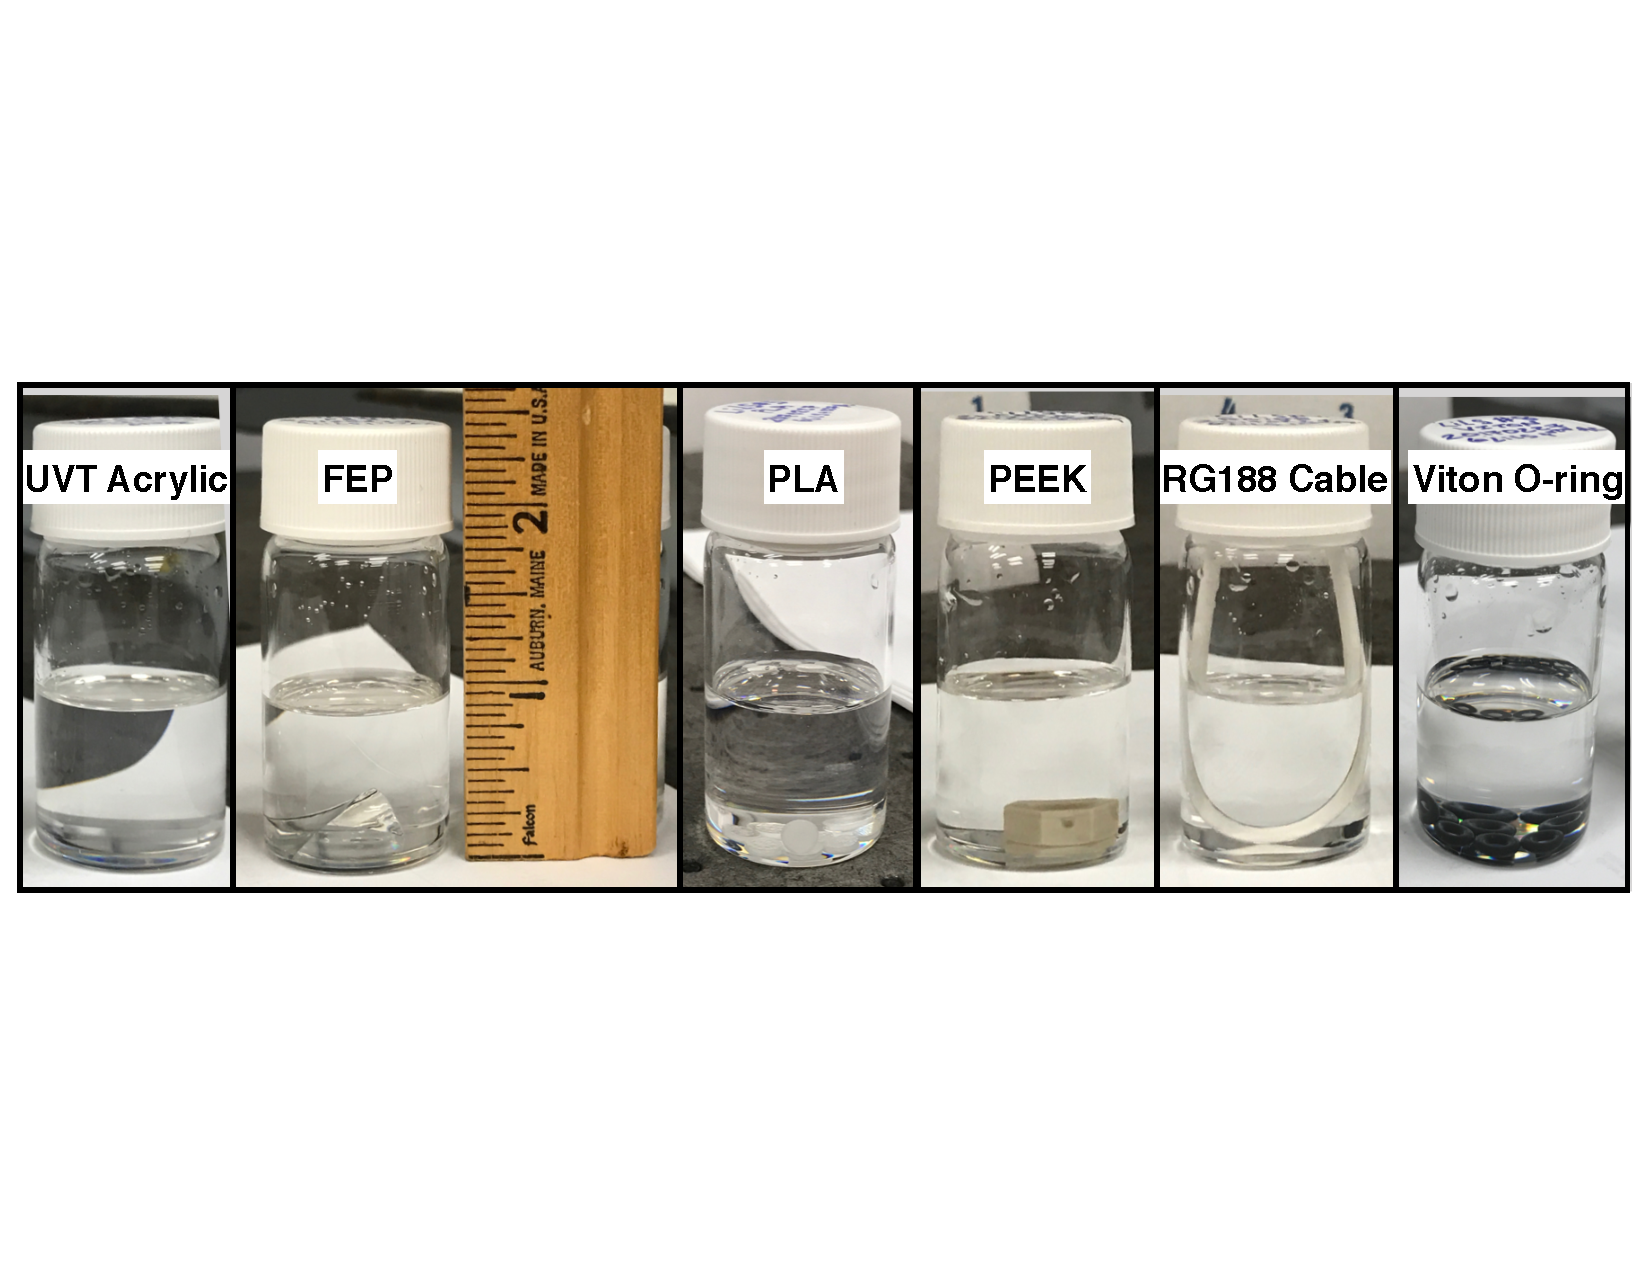
\includegraphics[width=0.8\linewidth]{tex/6-ac227-images/BNL/Samples}
	\caption[Material sample vials]{Photos of all material sample vials filled with \Ac spiked LiLS, with ruler for scale.}	
	\label{fig:samples}
\end{figure}

\subsection{Detector}

The detector consisted of a 2'' photomultiplier tube coupled using optical grease to a solid cylinder of UVT acrylic painted white with an insert cut out to hold the sample vials, as shown in Figure~\ref{fig:blackbox}.
Placed in a dark box the PMT is cabled to a CAEN DT55xx Desktop HV Power Supply and a CAEN DT5730 8 Channel 14-bit 500 MS/s Digitizer \cite{CAENDigit}.
A modified version of Wavedump 3.7.2 \cite{CAENWD} was used to start and stop the data runs and save the waveforms of the signals.

\begin{figure}[H]
	\centering
	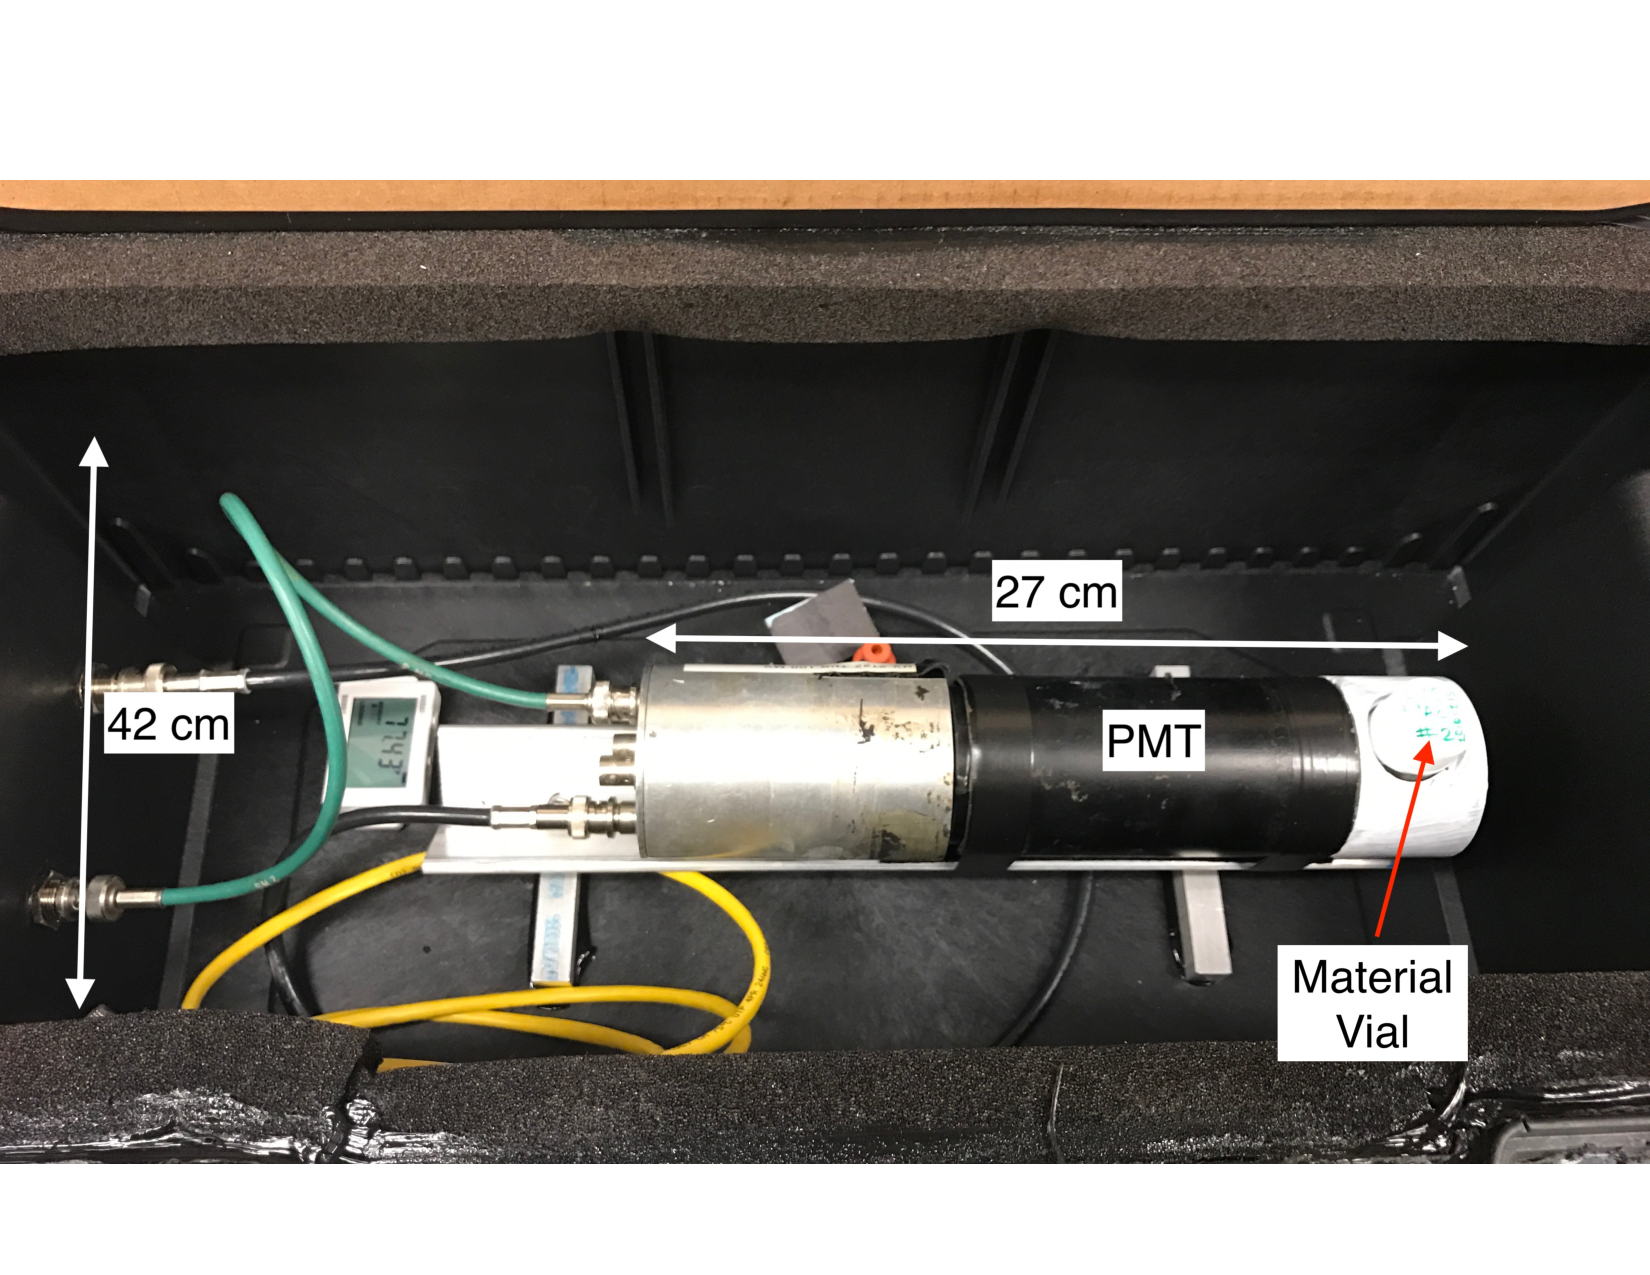
\includegraphics[width=0.7\linewidth]{tex/6-ac227-images/BNL/BlackBox}
	\caption[Detector used for material adsorption studies]{Detector used for material studies, consisting of a 2'' PMT coupled to an acrylic cylinder holding the sample vials, all contained in a dark box. The PMT is cabled to a power supply and digitizer that exist outside of the box.}
	\label{fig:blackbox}
\end{figure}

\subsection{Data Analysis}

The raw waveforms are analyzed to calculate the energy, PSD, and time of each signal. 
The energy is determined by taking an integral of the waveform in ADC units and then converted to nC by... 
The PSD is defined as... \todo{DEFINE these values}

The \Ac coincident alpha events, labeled RnPo events for the remainder of this document, are found by applying a set of timing, energy, and PSD cuts along with an accidental background subtraction.
Po events are found first by applying the energy and PSD cuts listed in Tabel~\ref{tab:MatCuts}. 
Rn coincidental events are found by looking in a 12.85 ms time window before a given Po event and applying the same energy and PSD cuts.
This time window is 5 times the lifetime of Po, 2.57 ms, allowing the collection of all possible coincident events.
Accidental events are found by looking in the same length time window, using the same energy and PSD cuts, but offset 10 Po lifetimes before a given Po event.
RnPo events are then found by subtracting the accidental events from the coincident events.
See Figure~\ref{fig:rnpoenpsd} for an example of typical energy and PSD distributions.

\begin{table}[H]
	\centering
	\begin{tabular}{c|c}
		\hline 
		Energy & 0.01 $<$ E $<$ 0.055 nC \\ 
		\hline 
		PSD & 0.31 $<$ PSD $<$ 1.0  \\ 
		\hline 
		$\Delta$t = t$_{\mathrm{delay}}$ - t$_{\mathrm{prompt}}$ & $\Delta$t $<$ 5$\tau_{\textrm{Po}}$ \\ 
		\hline 
	\end{tabular} 
	\caption{Energy, PSD, and time cuts used to find RnPo events where $\tau_{\textrm{Po}}$ = 2.57 ms. Energy and PSD cuts are applied to both prompt and delay events.}
	\label{tab:MatCuts}
\end{table}

\begin{figure}[H]
	\centering
	\begin{subfigure}{0.5\linewidth}
		\centering
		\includegraphics[width=1.\linewidth]{"tex/6-ac227-images/BNL/RnPoEn_TimeBin23_S2"}
		\caption{}
	\end{subfigure}%
	\begin{subfigure}{0.5\linewidth}
		\centering
		\includegraphics[width=1.\linewidth]{"tex/6-ac227-images/BNL/RnPoPSD_TimeBin23_S2"}
		\caption{}
	\end{subfigure}
	\caption[Typical RnPo energy and PSD distributions]{Typical energy (a) and PSD (b) distributions for RnPo events in the reference sample after accidental background subtraction.}
	\label{fig:rnpoenpsd}
\end{figure}

The rate of RnPo events is measured by fitting the RnPo $\Delta$t distribution with
\begin{equation}
	f(t) = N_0e^{-t/\tau}
	\label{eq:MatDtFit}
\end{equation}
where $N_0$ and $\tau$, the lifetime of \Po, are allowed to vary. 
Using the fit results, the rate is then defined as
\begin{equation}
	R = \frac{N_0 \tau}{\textrm{bin-width}\times\textrm{livetime}}
\end{equation}
\begin{equation}
	\sigma_R = R \times \sqrt{  \left(\frac{\sigma_{N_0}}{N_0}\right)^2 + \left(\frac{\sigma_{\tau}}{\tau}\right)^2 + \frac{2\sigma_{N_{0}\tau}}{N_0\tau} }
\end{equation}
where the livetime is measured, for each run, as the time from the beginning of the run to the last Po event. 
An example of a typical RnPo $\Delta$t distribution can be seen in Figure~\ref{fig:rnpodttimebin23s2}. It should be noted here that the energy and PSD cuts were made wide enough so that no efficiency correction needed to be applied.

\begin{figure}[H]
	\centering
	\includegraphics[width=1.\linewidth]{"tex/6-ac227-images/BNL/RnPoDt_TimeBin23_S2"}
	\caption[Typical RnPo $\Delta$t distribution]{A typical example of the RnPo $\Delta$t distributions for the reference sample. Left: coincidental and accidental distributions found using the defined energy and PSD cuts. Right: the $\Delta$t distribution after subtraction of the accidental distribution, fit with Equation~\ref{eq:MatDtFit}.}
	\label{fig:rnpodttimebin23s2}
\end{figure}

\subsection{Results}

The RnPo rate was calculated for each material sample and the reference sample over a period of about six months. These results can be seen in Figure~\ref{fig:ratevstimeallsamples}.
Though statistical errors vary from around 0.6-1\%, overall rates vary at a rate of around 12\%, indicating systematic variations.

\begin{figure}[H]
	\centering
	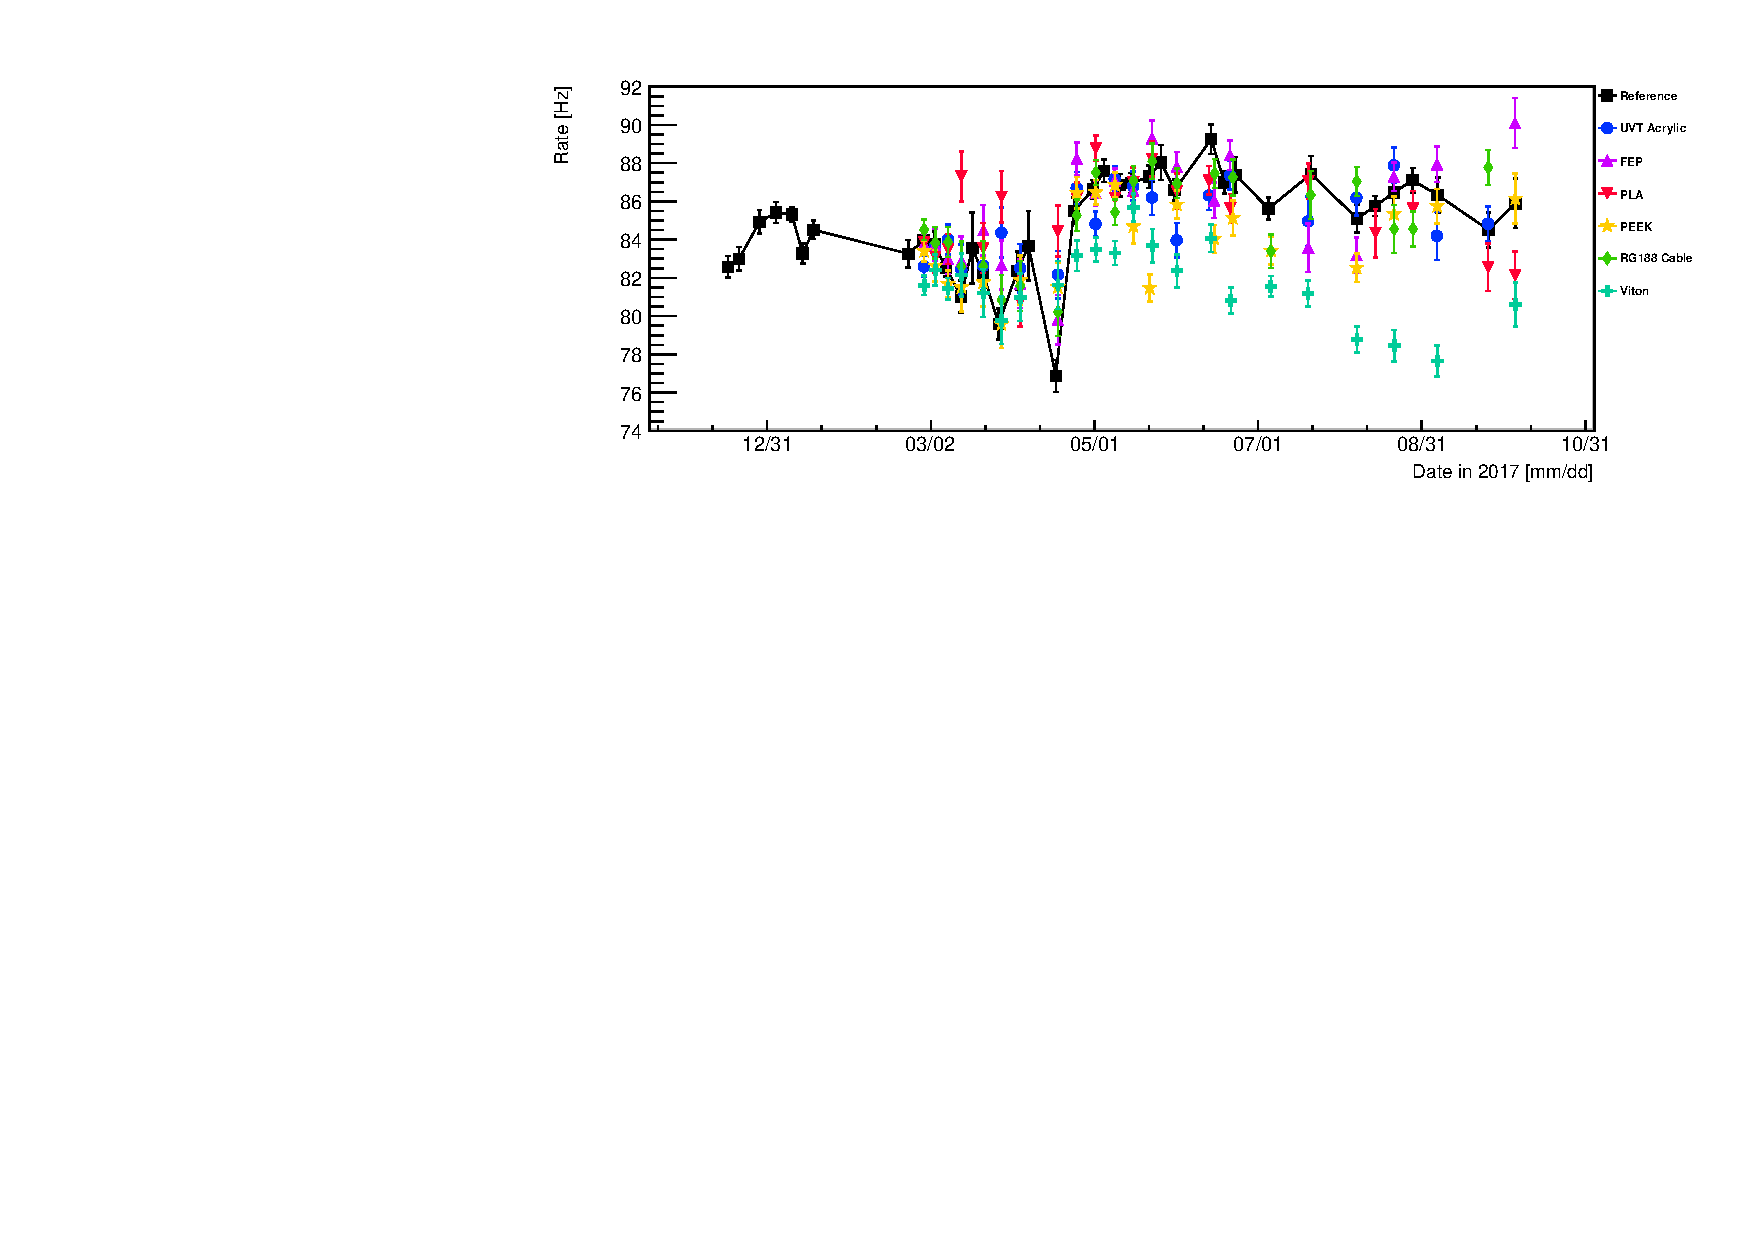
\includegraphics[width=1\linewidth]{tex/6-ac227-images/BNL/RateVsTime_AllSamples}
	\caption[\Ac rate for each material sample]{\Ac rate for each material sample. Errors are statistical.}
	\label{fig:ratevstimeallsamples}
\end{figure}

Systematic variations can be better understood by looking at the behavior of the Po energy distribution through time.
This was done by fitting this distribution for the reference sample with a sum of two Gaussians to account for the non-Gaussian nature of the peak as demonstrated in Figure~\ref{fig:poenfittimebin23s2}.
The mean and 1$\sigma$ width of each of these Gaussians is show in Figures~\ref{fig:poenmeanvstimes2} and ~\ref{fig:poenwidthvstimes2}.
It can be seen that the \Po energy mean varies about 5\% and the width around 15\%.

The amount of variation seen in measured rates and the \Po energy distribution, indicates that the system is not repeatable and introduces significant systematic errors. 
Though the PMT and acrylic holder were glued in place, the sample vials were repeatedly removed and replaced, possibly shifting the placement of the acrylic holder and the optical grease.
If the experiment were to be repeated a more robust detector system would be needed to eliminate these systematic errors.

\begin{figure}[H]
	\centering
	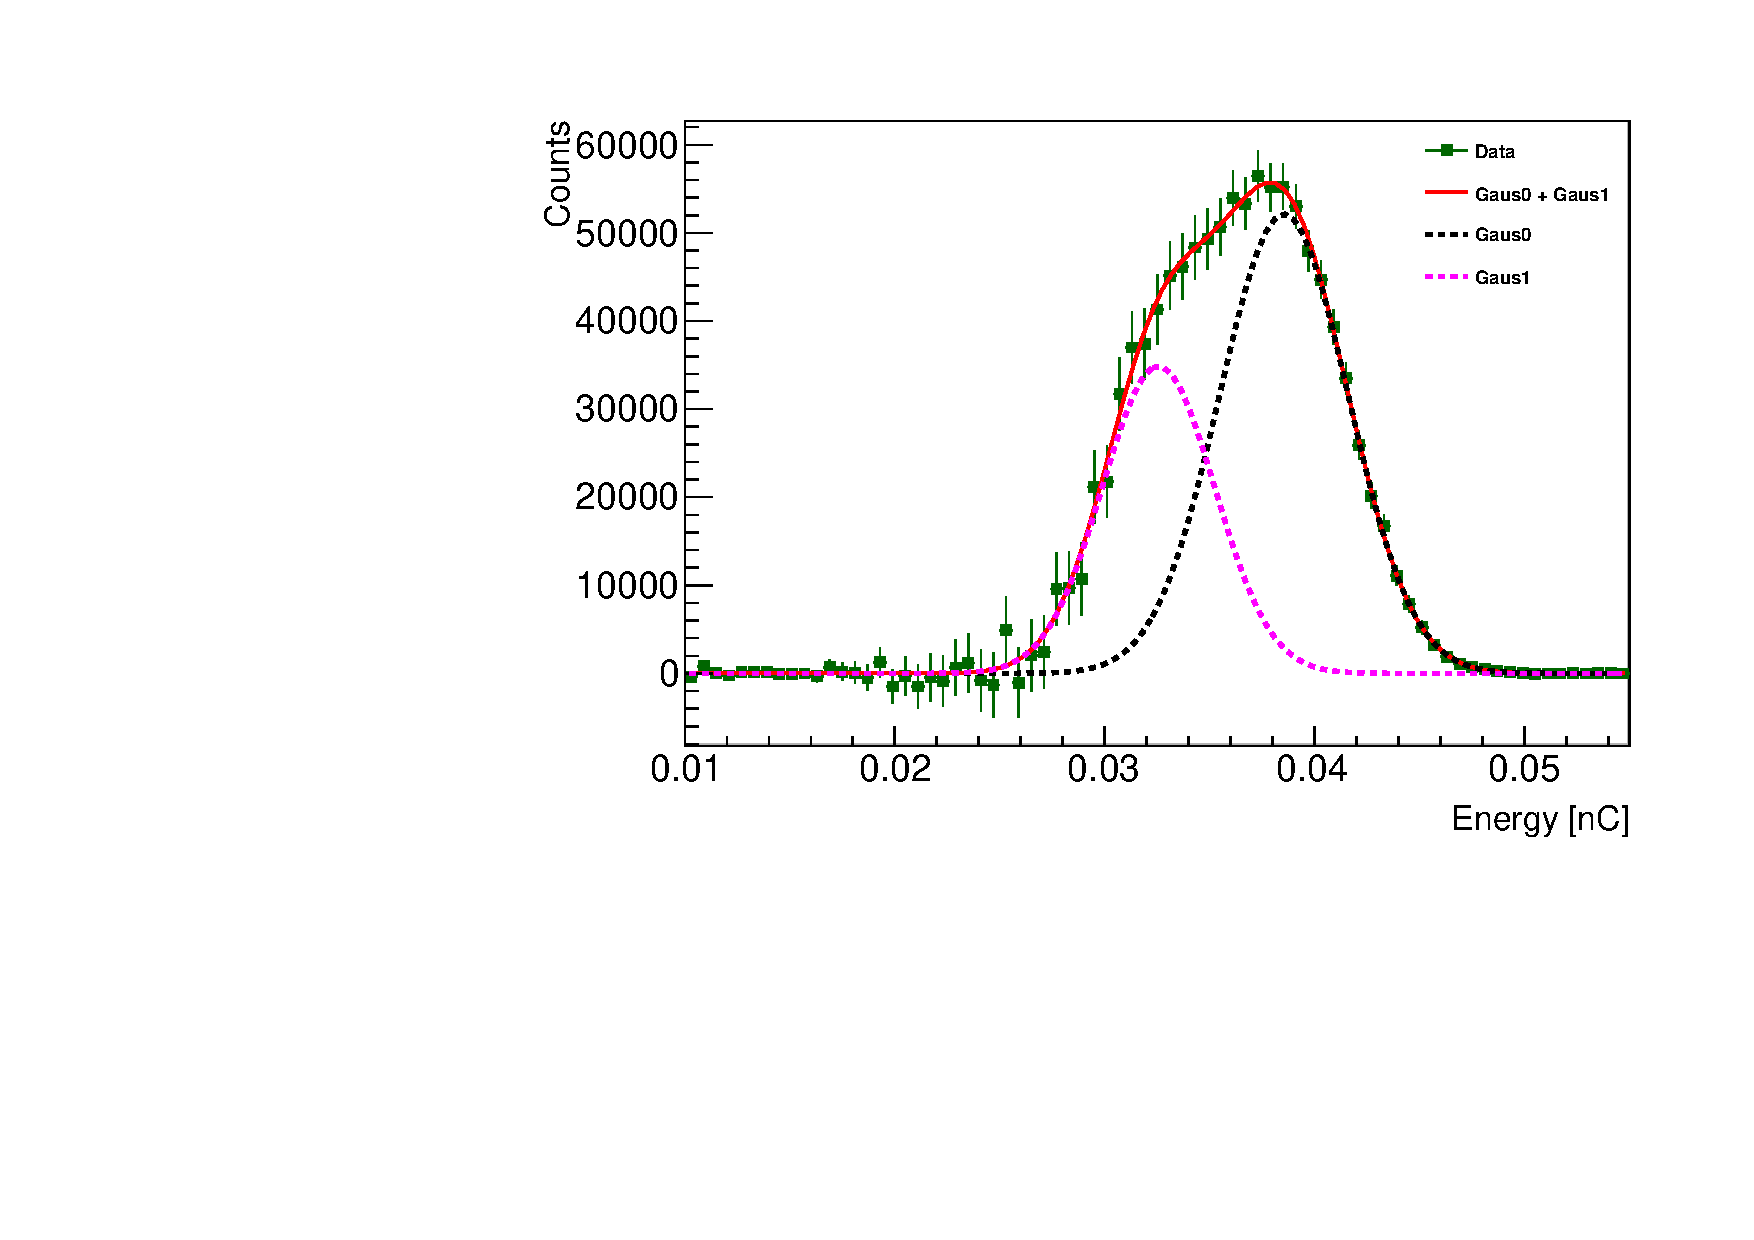
\includegraphics[width=0.6\linewidth]{tex/6-ac227-images/BNL/PoEnFit_TimeBin23_S2}
	\caption[\Po energy distribution for reference sample with two Gaussian fit]{\Po energy distribution for the reference sample, fit with a sum of two Gaussians. The total fit is seen in red, while the two Gaussians are drawn as the pink and black dashed lines.}
	\label{fig:poenfittimebin23s2}
\end{figure}

\begin{figure}[H]
	\centering
	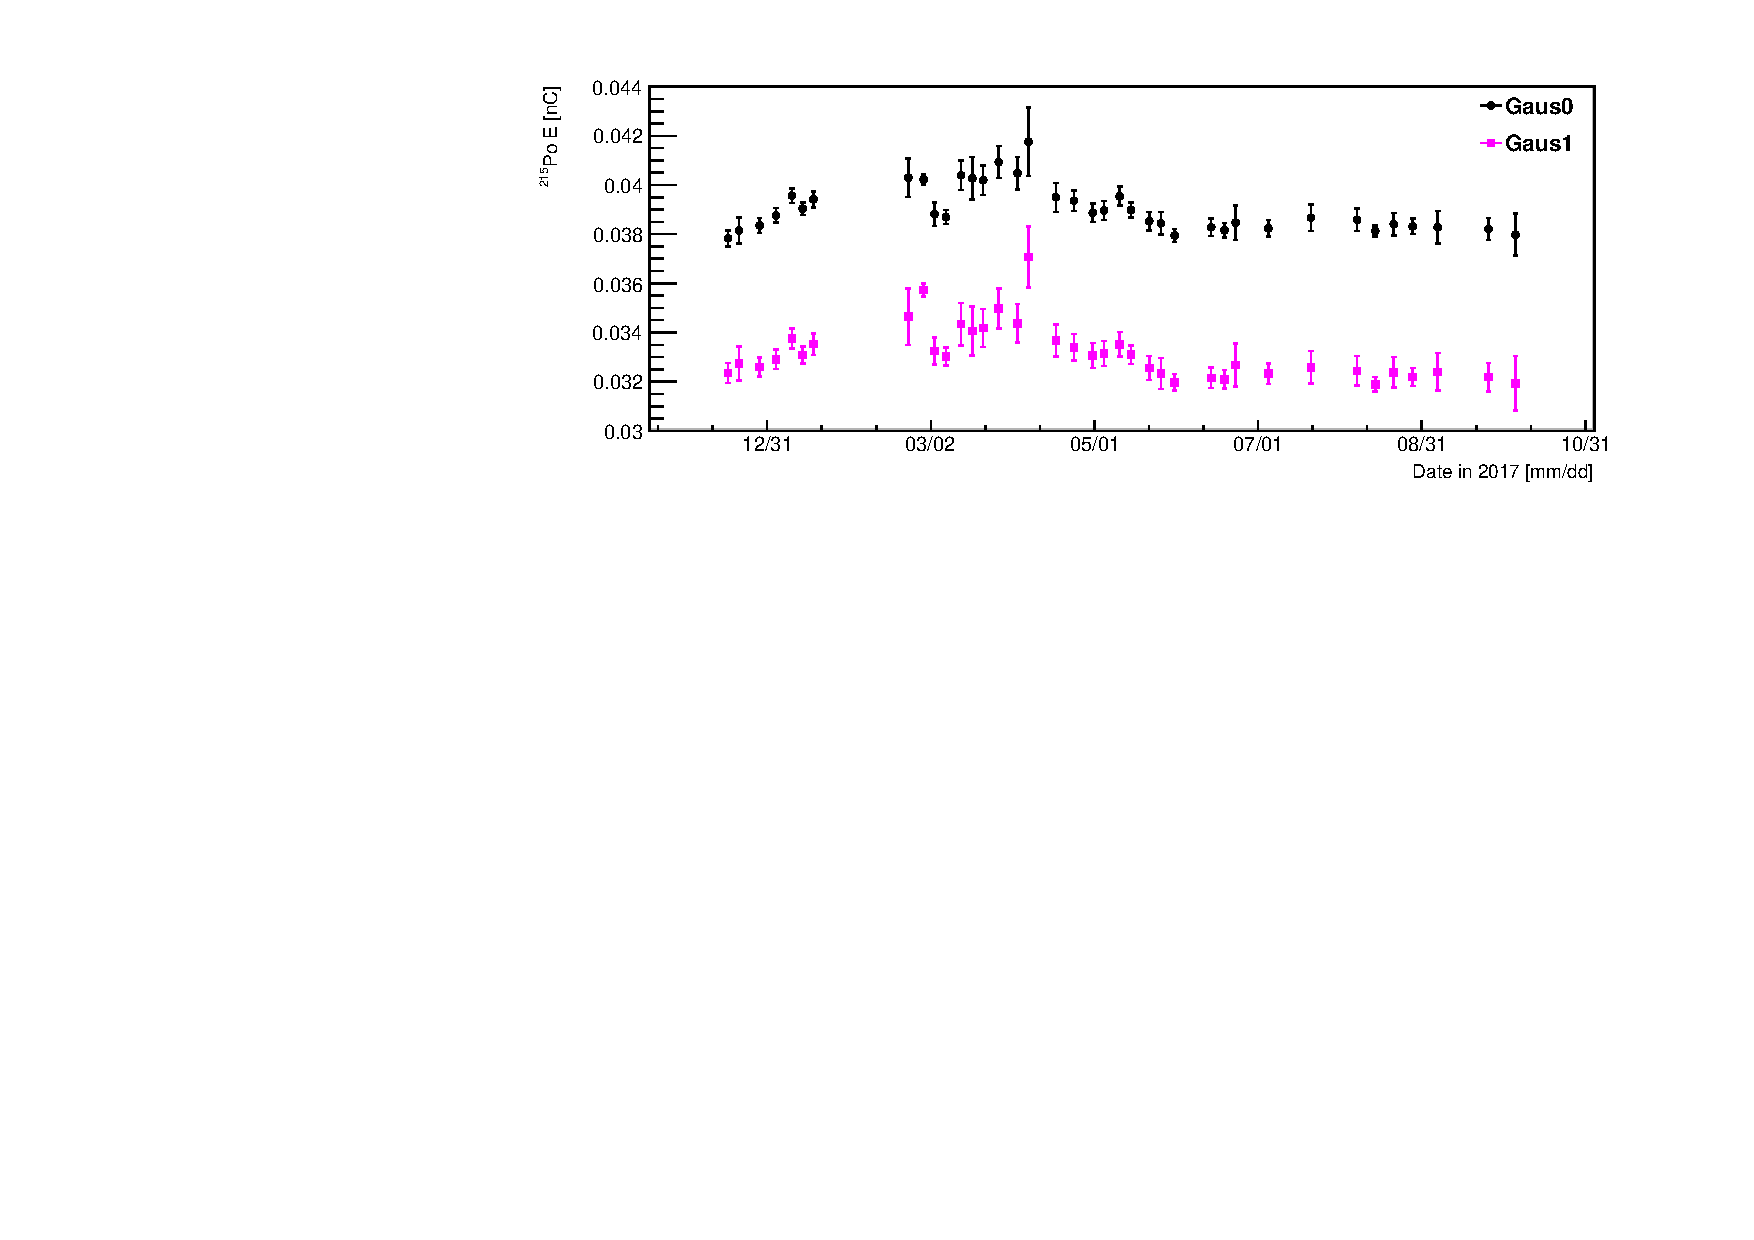
\includegraphics[width=0.8\linewidth]{tex/6-ac227-images/BNL/PoEnMeanVsTime_S2}
	\caption[\Po mean versus time for the reference sample]{The mean of the two Gaussians fit to the \Po distribution for the reference sample.}
	\label{fig:poenmeanvstimes2}
\end{figure}

\begin{figure}[H]
	\centering
	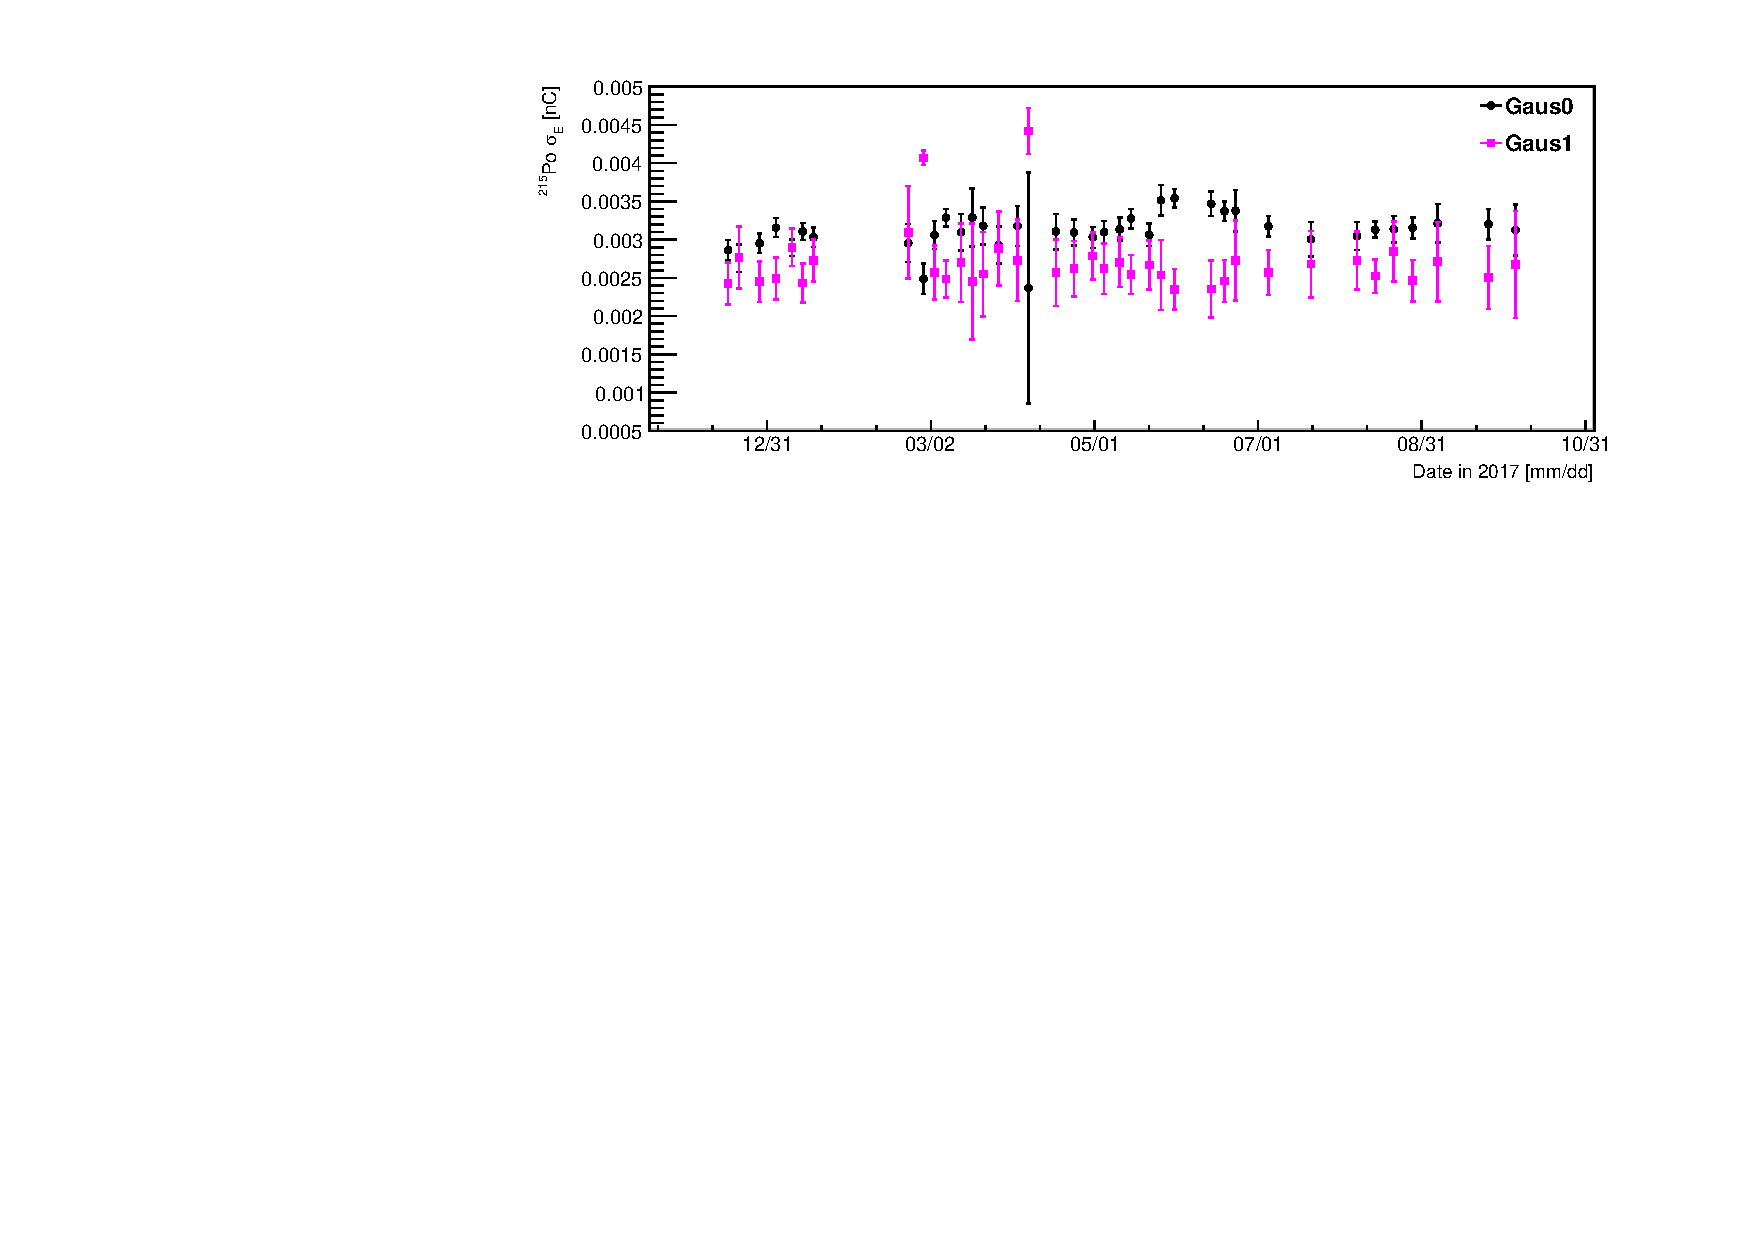
\includegraphics[width=0.8\linewidth]{tex/6-ac227-images/BNL/PoEnWidthVsTime_S2}
	\caption[\Po 1$\sigma$ width versus time for the reference sample]{The 1 $\sigma$ width of the two Gaussians fit to the \Po distributions for the reference sample.}
	\label{fig:poenwidthvstimes2}
\end{figure}

\begin{figure}[H]
	\centering
	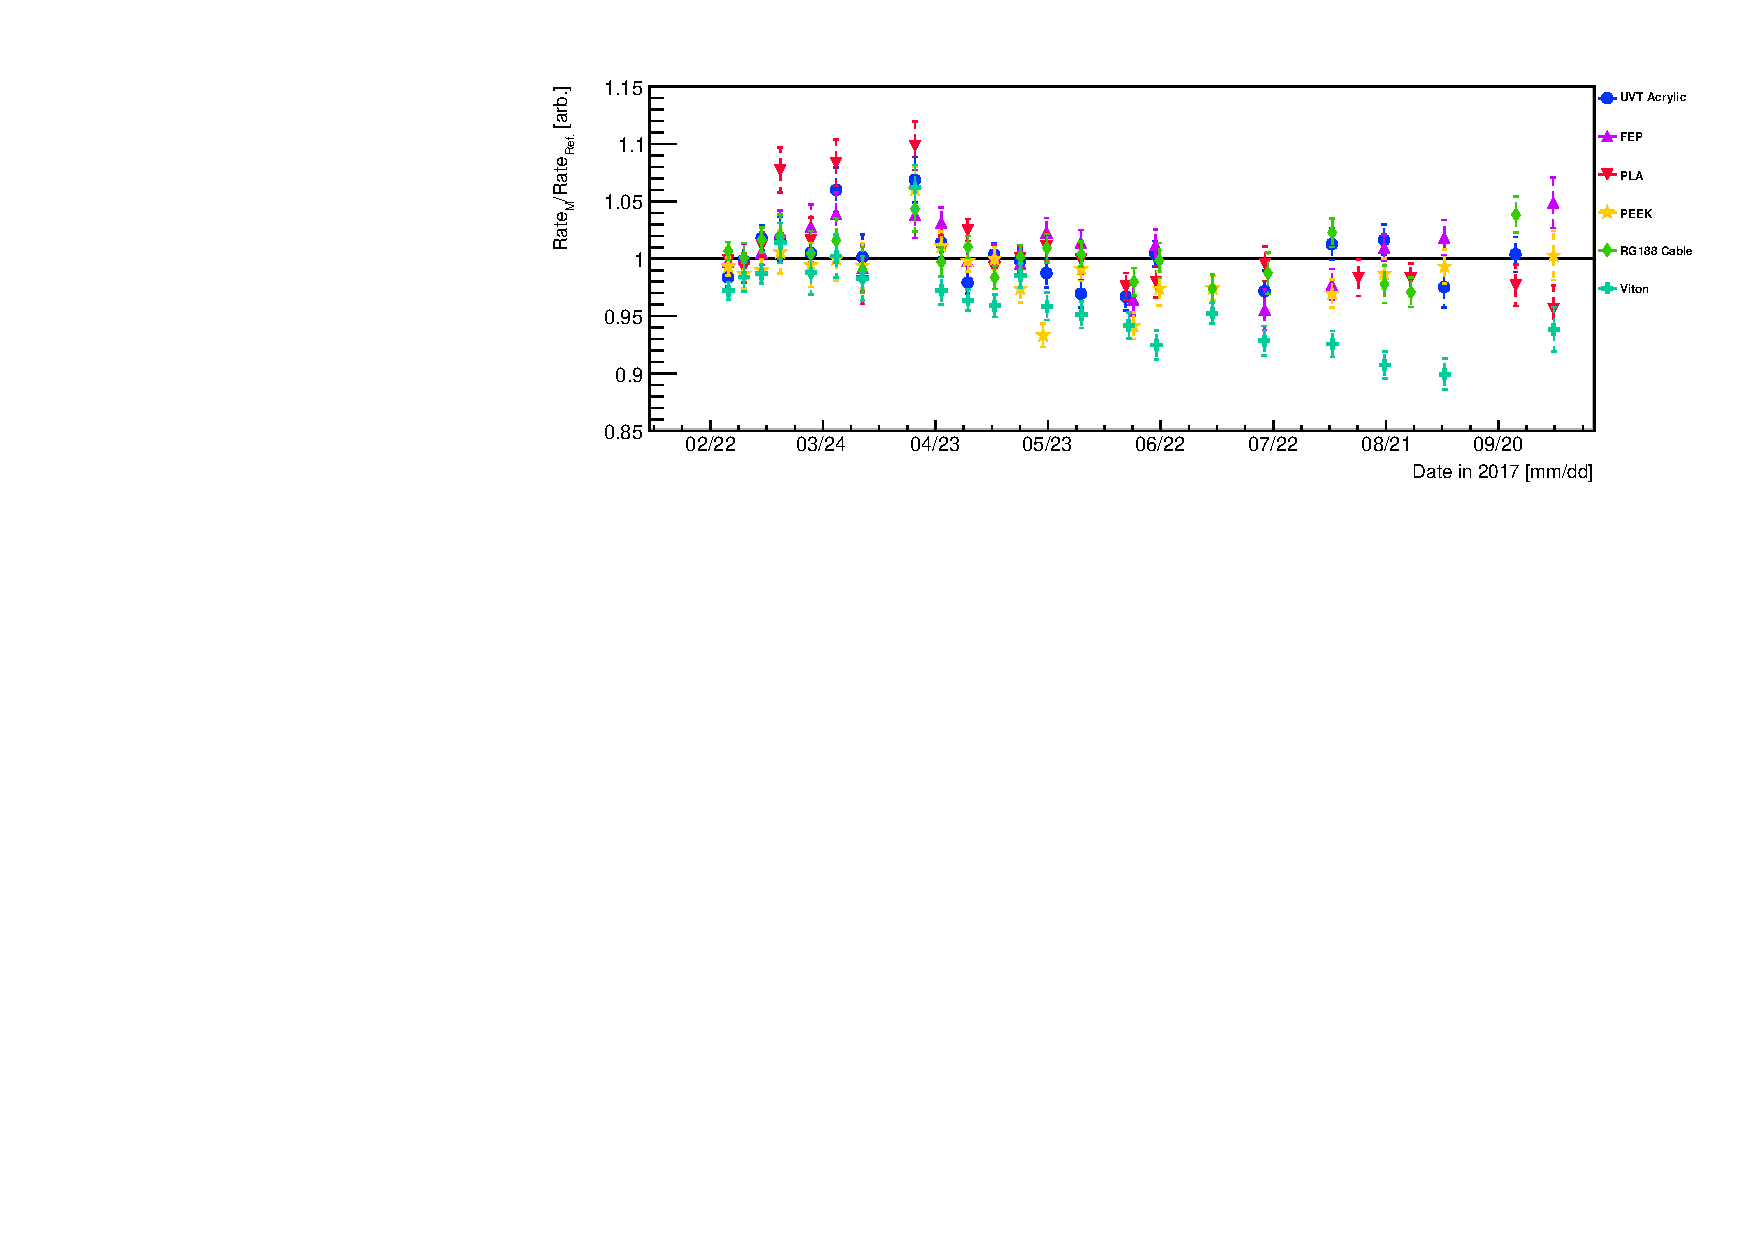
\includegraphics[width=1\linewidth]{tex/6-ac227-images/BNL/RelRateVsTime_AllSamples}
	\caption[\Ac rate for each material sample relative to the reference sample]{\Ac rate for each material sample relative to the reference sample.}
	\label{fig:relratevstimeallsamples}
\end{figure}

\begin{table}[H]
	\centering
\begin{tabular}{|c|c|c|}
	\hline 
	\textbf{Material} & \textbf{Constant} & \textbf{$\chi^2$/NDF} \\ 
	\hline 
	UVT Acrylic  & 0.997 $\pm$ 0.003 & 56.5/20 = 2.82 \\ 
	\hline 
	FEP & 1.005 $\pm$ 0.003 & 44.1/20 = 2.21 \\ 
	\hline 
	PLA & 1.003 $\pm$ 0.003 & 80.6/20 = 4.03 \\ 
	\hline 
	PEEK & 0.985 $\pm$ 0.003 & 70.9/20 = 3.55 \\ 
	\hline 
	RG188 Cable & 1.001 $\pm$ 0.003 & 38.3/21 = 1.82 \\ 
	\hline 
	Viton  & 0.960 $\pm$ 0.002 & 136.3/21 = 6.49 \\ 
	\hline 
\end{tabular} 
\caption{The results of fitting the relative rate for each material sample with a constant.}
\label{tab:MatFitC}
\end{table}

\begin{table}[H]
	\centering
\begin{tabular}{|c|c|c|c|}
	\hline 
	\textbf{Material} & \textbf{Constant} & \textbf{Slope [ratio/yr]} & \textbf{$\chi^2/NDF$} \\ 
	\hline 
	UVT Acrylic  & 1.5 $\pm$ 0.8 & -0.01 $\pm$ 0.02 & 56.2/19 = 2.96 \\ 
	\hline 
	FEP  & 1.3 $\pm$ 0.8 & -0.005 $\pm$ 0.018 & 44.0/19 = 2.32 \\ 
	\hline 
	PLA  & 4.4 $\pm$ 0.8 & -0.07 $\pm$ 0.02 & 64.3/19 = 3.38 \\ 
	\hline 
	PEEK  & 2.9 $\pm$ 0.8 & -0.04 $\pm$ 0.02 & 65.2/19 = 3.43 \\ 
	\hline 
	RG188 Cable  & 2.3 $\pm$ 0.8 & -0.03 $\pm$ 0.02 & 35.7/20 = 1.79\\ 
	\hline 
	Viton  & 7.7 $\pm$ 0.7 & -0.14 $\pm$ 0.02 & 48.9/20 = 2.45 \\ 
	\hline 
\end{tabular} 
\caption{The results of fitting the relative rate for each material with a straight line.}
\label{tab:MatFitLine}
\end{table}

\begin{figure}[H]
	\centering
	\includegraphics[width=1.\linewidth]{"tex/6-ac227-images/BNL/RnPoEn_FirstAndLast_S8"}
	\caption{}
	\label{fig:rnpoenfirstandlasts8}
\end{figure}

\begin{figure}[h]
	\centering
	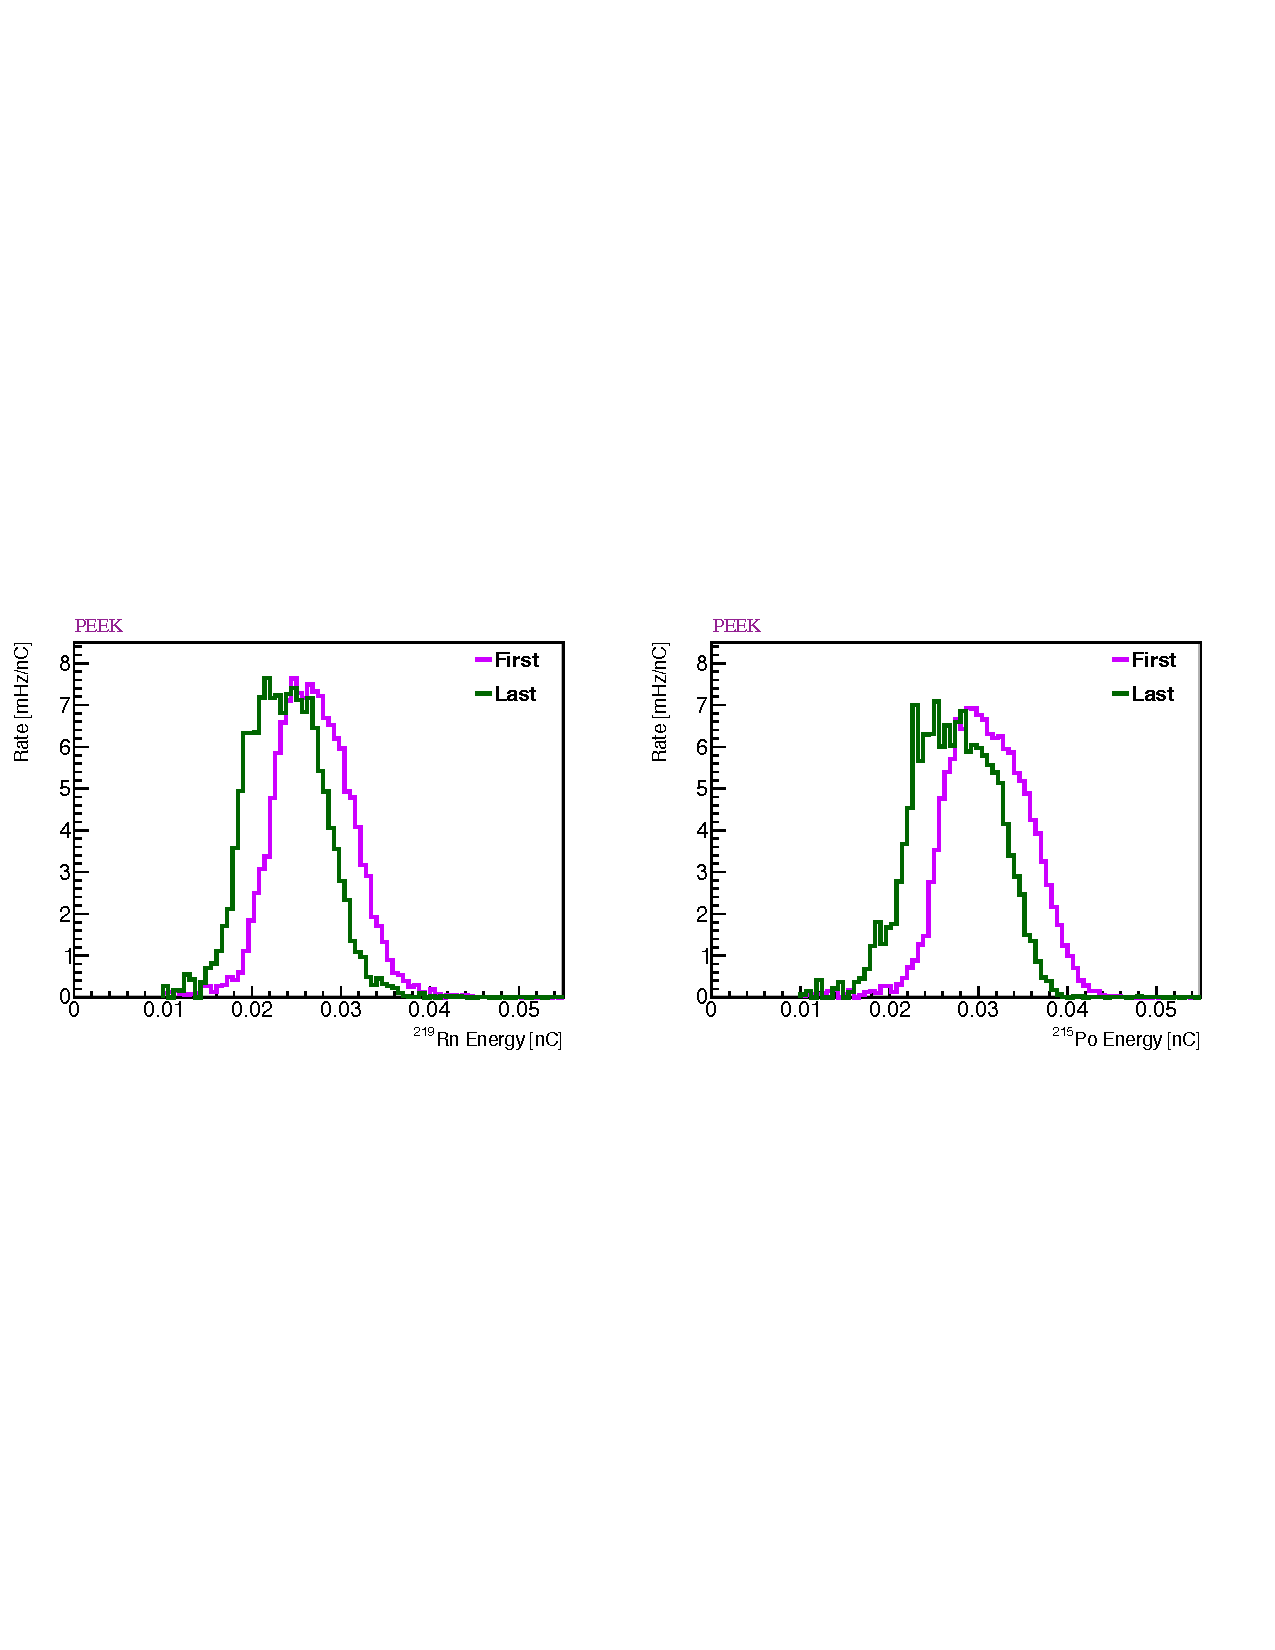
\includegraphics[width=1\linewidth]{tex/6-ac227-images/BNL/RnPoEn_FirstAndLast_S6}
	\caption{}
	\label{fig:rnpoenfirstandlasts6}
\end{figure}





\section{Event Selection in the PROSPECT AD}

\section{Detector Stability Results}

\section{Volume Variation Results}

